\section{Experiments} \label{sec:experiment}
In this section, we measure the overall performance of the optimized 
OpenCL based BFS accelerator on Intel Xeon-FPGA, a closely coupled CPU-FPGA
architecture, over a set of representative graphs. Then we compare the 
resulting accelerator to the reference design in an HLS benchmark Spector.

\subsection{Experiment Setup}
The graph benchmark used in this work includes three real-world graphs and 
two synthetic graphs generated using R-MAT model \cite{chakrabarti2004rmat} 
as listed in Table \ref{tab:graph}. The real-world graphs are from social network \cite{yang2012defining, 
leskovec2009community, takac2012data} while the R-MAT graphs are generated 
using the Graph 500 benchmark parameters ($A=0.59, B=0.19, C=0.19$). To make the 
presentation easier, the five benchmark graphs are shorted as YT, 
LJ, Pokec, R-MAT\uppercase\expandafter{\romannumeral1}, 
R-MAT\uppercase\expandafter{\romannumeral2} respectively. We refer 
to an R-MAT graph with scale $S$ ($2^{S}$ nodes) and edge factor $E$ ($E\times 2^{S}$). 
In the experiments, we averaged 64 BFS with random starting points. 
In order to avoid trivial search, we remove the BFS with less than 3 levels.

\begin{table}
    \centering
  \caption{Graph Benchmark}
  \label{tab:graph}
  \begin{tabular}{cccc}
    \toprule
      Name & \# of vertex & \# of edge & Type \\
    \midrule
      YT \cite{yang2012defining} & 1157828 & 2987624 & Undirectional \\
      LJ \cite{leskovec2009community} & 4847571 & 68993773 & Directional \\
      PK \cite{takac2012data} & 1632804 & 30622564 & Directional \\
      R-MAT\uppercase\expandafter{\romannumeral1} & 524288 & 16777216 & Directional \\
      R-MAT\uppercase\expandafter{\romannumeral2} & 2097152 & 67108864 & Directional \\
  \bottomrule
\end{tabular}
\vspace{-1em}
\end{table}

\subsection{Performance evaluation}
\subsubsection{Overall performance}
We use the million traverse per second (MTEPS) as 
the performance metric. The performance of the proposed BFS 
accelerator on the graph benchmark is 
presented in Table \ref{tab:performance-summary}. 
It gets up to 817.5 MTEPS on the R-MAT\uppercase\expandafter{\romannumeral2}
and achieves 508.1 MTEPS on average. When compared to the reference BFS 
implementation in Spector, the proposed design shows 5.5X and 10.3X 
speedup on YT graph and R-MAT\uppercase\expandafter{\romannumeral1} 
graph respectively while Spector fails on the other three graphs with larger data sets 
because of bugs in the code. In general, the proposed design performs better on 
R-MAT graphs with higher average degree. On the contrast, YT with 
low average degree suffers higher reordering and batching cost. In addition, 
YT is an undirectional graph while the accelerator takes each edge as bidirectional ones. 
Therefore, this also leads to relatively lower MTEPS in the experiments. 
\begin{table}
    \centering
  \caption{Performance summary}
  \label{tab:performance-summary}
  \begin{tabular}{cccccc}
    \toprule
      Benchmark & YT & LJ & Pokec & R-MAT\uppercase\expandafter{\romannumeral1} & R-MAT\uppercase\expandafter{\romannumeral2} \\
    \midrule
      MTEPS & 65.7 & 517.4 & 478.0 & 661.9 & 817.5 \\
      Speedup & 5.5X & - & - & 10.3X & - \\
  \bottomrule
\end{tabular}
\vspace{-1em}
\end{table}

The proposed design needs a coupled CPU to reorganize the RPA based on the frontier vertices.
The process has a lot of random access and it is appropriate for CPU because 
of the optimized cache sub system. To evaluate the approach, we further analyze the 
execution time distribution of the BFS. According to Figure \ref{fig:runtime}, the CPU execution time 
takes a small proportion of the whole execution time in general, while the proportion is relatively 
higher for the social network graphs which have deeper levels and more processing on CPU 
compared to the R-MAT graphs. 
\begin{figure}
	\center{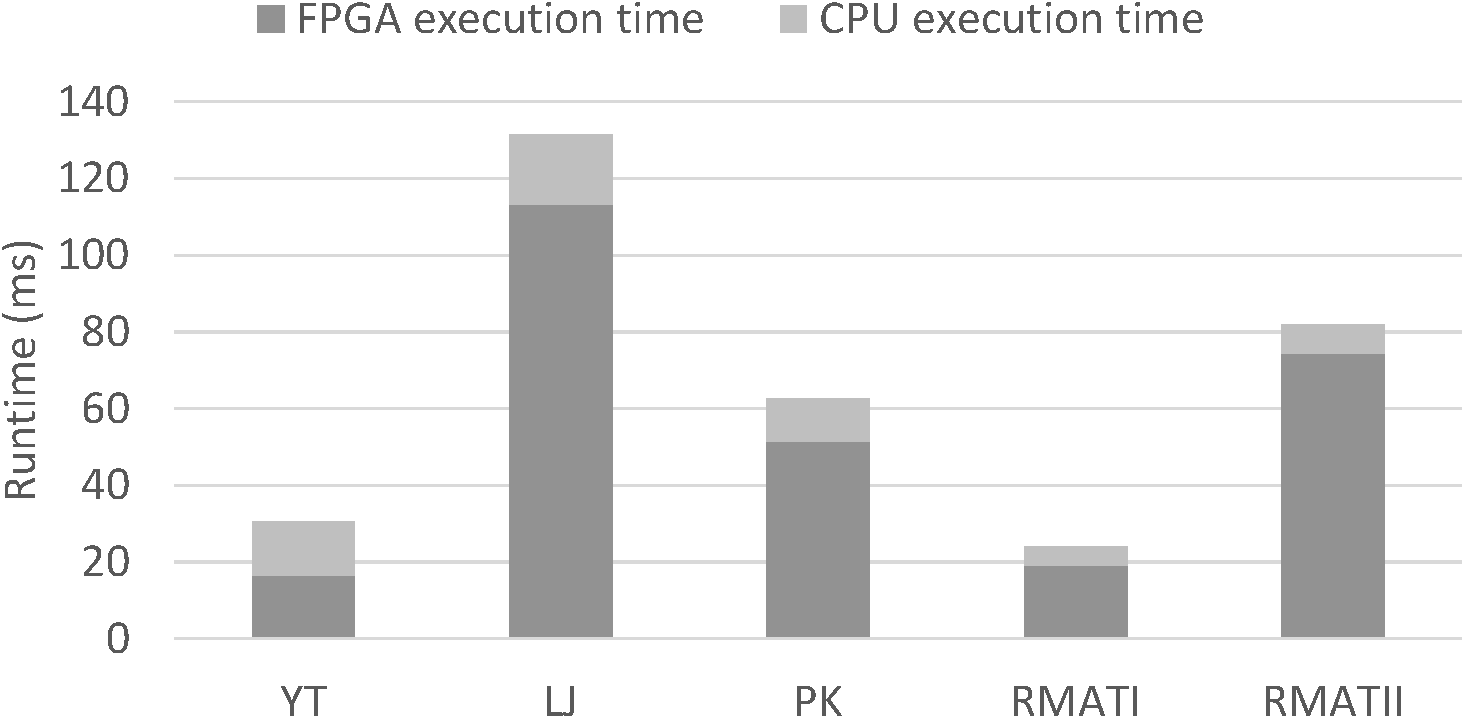
\includegraphics[width=0.85\linewidth]{runtime}}
    \caption{Runtime distribution of the BFS accelerator on different graphs}
\label{fig:runtime}
\vspace{-1em}
\end{figure}

\subsubsection{Performance comparison}
On top of the comparison to the reference OpenCL design, we also compare 
this work to a set of existing BFS accelerators on FPGAs. As the platforms 
and graph benchmark used in these work are mostly different, it is 
difficult to make a completely fair end-to-end comparison. 
A rough comparison result is listed in Table \ref{tab:compare}. It can be found that the OpenCL
based BFS accelerator proposed in this work achieves comparable performance to many 
prior hand crafted design and even outperfroms some of them. When compared to design on high-end 
FPGA computing system with mutiple FPGAs like Convey HC2\cite{attia2014cygraph}, 
the overall performance in this work is still lower, 
but the performance per FPGA is better. In addition, the OpenCL based design 
gains the software-like features and can be easily ported to similar FPGA boards.

\begin{table}
  \caption{FPGA based BFS accelerator performance comparison}
  \label{tab:compare}
    \setlength{\tabcolsep}{4pt} % Default value: 6pt
    %\renewcommand{\arraystretch}{1.5} % Default value: 1
  \begin{tabular}{ccc}
    \toprule
	System & Platform & MTEPS/FPGA\\
    \midrule
	Betkaouis'work\cite{betkaoui2012reconfigurable} & Convey HC-2 & 400\\
	CyGraph\cite{attia2014cygraph} & Convey HC-2    & 478 \\
	Shijie's work \cite{zhou2017accelerating} & Harpv1 & 330 - 670 \\
	Jialiang's work\cite{zhang2017boosting} & AC-510 & 166 \\
	FPGP\cite{dai2016fpgp} & VC707 & 122 \\
	ForeGraph\cite{Dai2017foregraph} & VCU110 & 364 - 1069 \\
	this work (R-MAT Graph) & Harpv2 &  739.7\\
	this work (Social Network) & Harpv2 & 353.7 \\
  \bottomrule
\end{tabular}
\vspace{-1em}
\end{table}

\subsubsection{Optimization approach analysis}
As mentioned, we mainly apply four different approaches including graph reordering, on-chip buffer partition,  
, data reorganization and hype pipelining to optimize the OpenCL based BFS accelerator.
While the graph reordering and on-chip buffer partition are naturally combined, 
we have the two optimizations evaluated together. The performance improvement 
by gradually applying the optimizations as presented in Figure \ref{fig:opt-analysis}.
Note that the accelerators with different optimizations have 8Mb bitmap implemented.
Batch size is set to be 16.
It can be found that the graph reordering and on-chip buffer partition contributes most to the overall 
performance improvement. 8X speedup over the base design is achieved on R-MAT graphs. 
The performance improvement of data reorganization varies on different graphs. 
On LJ graph, over 50\% improvement is obtained. Hyper pipelining is also demonstrated to be 
beneficial particularly on social network graphs with deeper BFS levels. 5\% to 10\% performance 
improvement is gained while the benefit is trivial to R-MAT graphs.
 
When different optimizations are applied to the OpenCL based BFS accelerator, 
the resulting FPGA implementation frequency is also different. As labeled in 
Figure \ref{fig:opt-analysis}, the proposed optimizations that simplify the 
processing on FPGAs also produce higher hardware implementation frequency.
This is also part of the reasons of performance improvement. Note that the 
hyper pipelining are implemented on host processor, so the accelerator frequency 
remains unchanged.

\begin{figure}
	\center{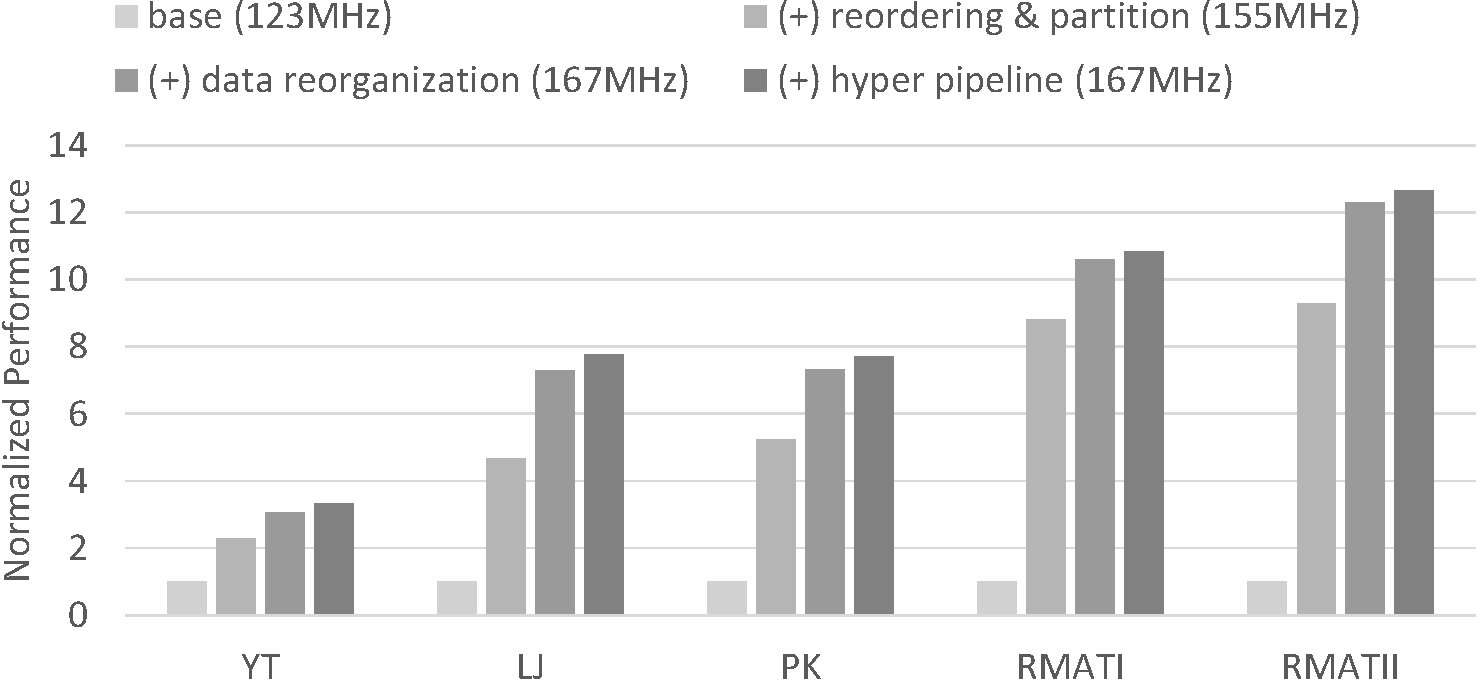
\includegraphics[width=0.85\linewidth]{opt-analysis}}
	\caption{Performance improvement with different high-level optimizations}
\label{fig:opt-analysis}
\vspace{-1em}
\end{figure}

\subsection{Batch trade-offs}
Graph reordering and batching contributes most to the BFS performance 
improvement and will be analyzed in this subsection. 
Figure \ref{fig:batch-perf} shows the BFS performance of different batch size.
In general, larger batch size induces higher performance and batch 16 
achieves the best performance on all the benchmark graphs. BFS performance 
starts to drop when the batch size is larger.  
\begin{figure}
	\center{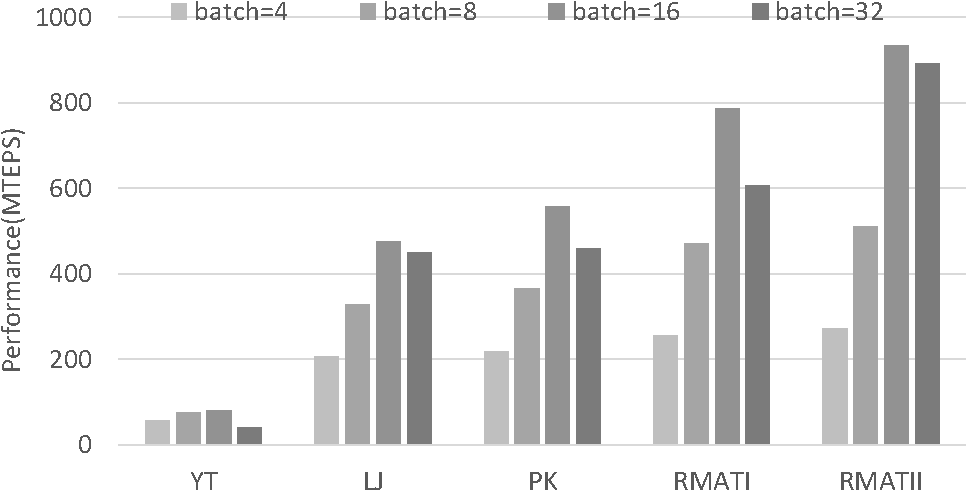
\includegraphics[width=0.8\linewidth]{batch-perf}}
    \caption{BFS performance of different batch size}
\label{fig:batch-perf}
\vspace{-1em}
\end{figure}


The proposed graph reordering and batching approach expands the 
graph layout and it will induce more memory overhead. The batch overhead 
on the benchmark graphs is illustrated in Figure \ref{fig:batch-overhead}. 
When the batch size increases, the CSR data increases accordingly. 
In general, to trade-off the batch overhead and the performance benefit, 
larger batch size is recommended for graphs with higher average degree 
and smaller batch size is better for graphs with lower degree 
such as YT. Given appropriate batch size setup, the data width 
of the edge access and the number of conflict-free parallel data paths 
in the BFS accelerator improves more significantly. 

\begin{figure}
	\center{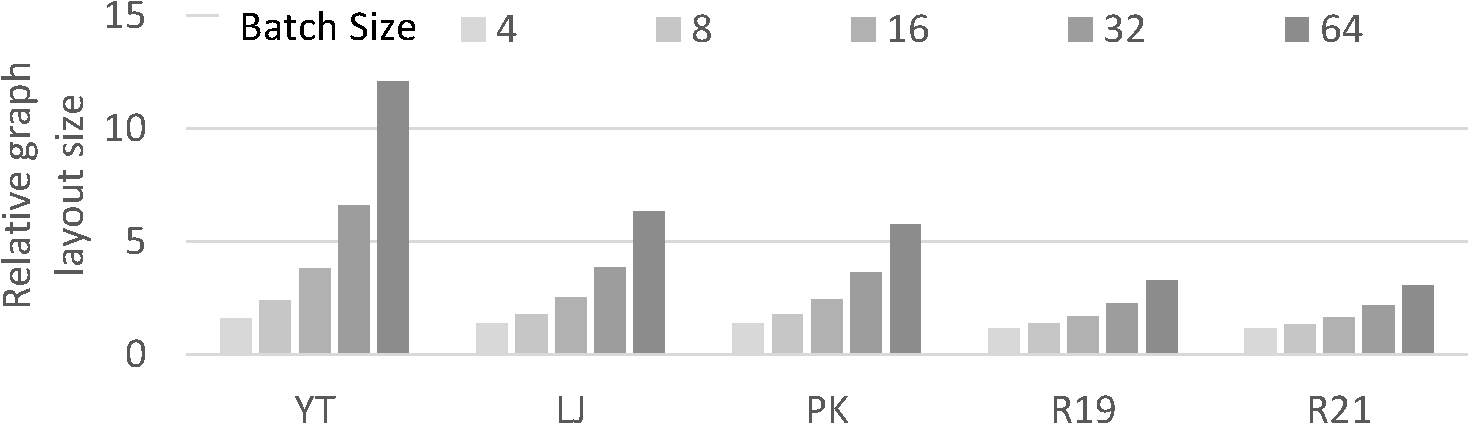
\includegraphics[width=0.95\linewidth]{batch-overhead}}
    \caption{Relative memory overhead of different batch size}
\label{fig:batch-overhead}
\vspace{-1em}
\end{figure}


The advantage of the batch is multi-folded and it is hard to 
quantify precisely as the benefits depend on the actual 
memory access sequence. Basically, batch mainly has the memory 
access coalesced and improves the memory bandwidth utilization, 
For sequential memory access and random access, 
we performed independent experiments on Harp-v2 
to evaluate the benefits. We measured the transfer time 
of 64MB data in different batch size and calculated the 
corresponding bandwidth. The bandwidth is normalized to 
the transfer with 32-bit data width. The relative bandwidth result is presented in 
Figure \ref{fig:mem-bandwidth}. Note that dependent random access pattern 
refers to the random accesses that can only proceed one after another.
This happens in the OpenCL based BFS. As low-degree frontier 
vertices in each data path traverse sequentially because the compiler 
has no clue if there is data dependency between different frontier 
neighbors. 

\begin{figure}
	\center{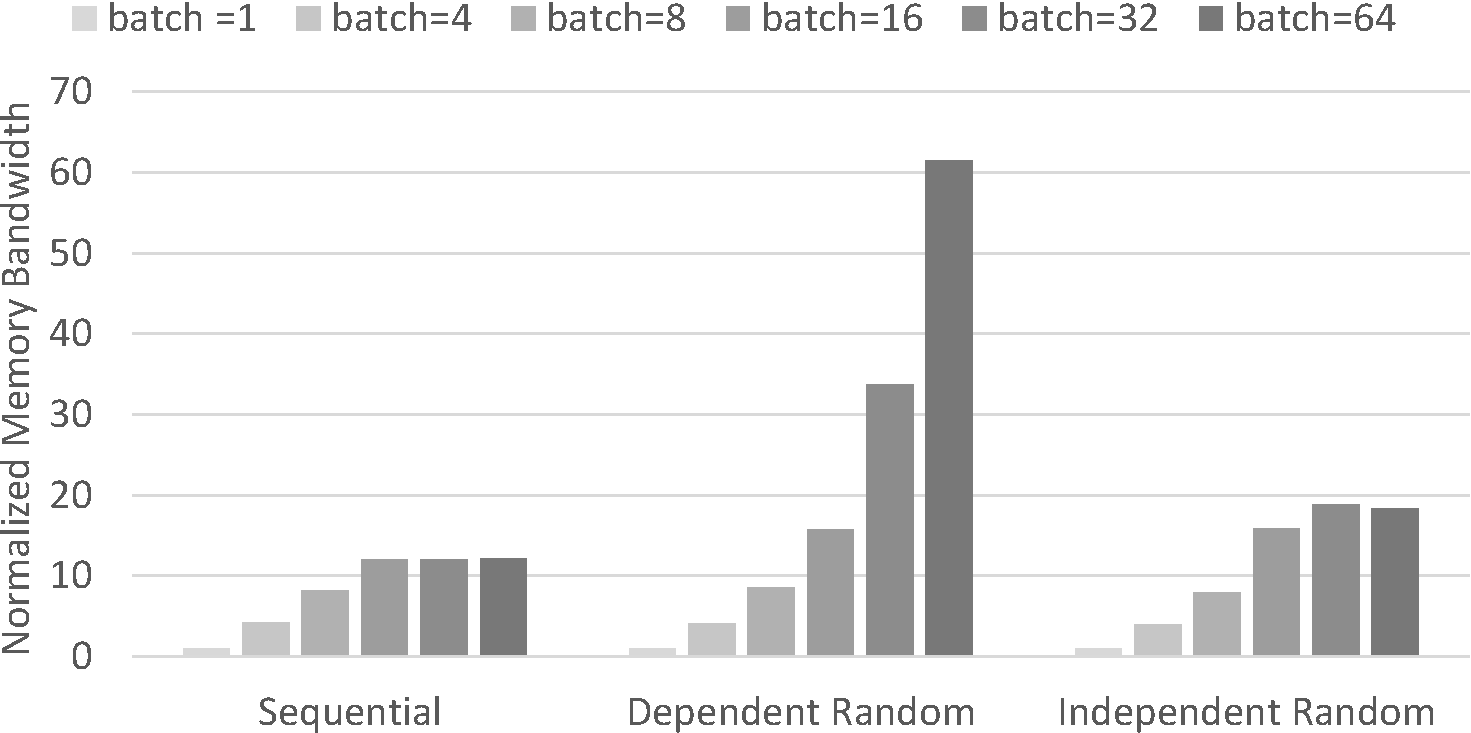
\includegraphics[width=0.85\linewidth]{mem-bandwidth}}
    \caption{Batch size influence on memory bandwidth}
\label{fig:mem-bandwidth}
\vspace{-1em}
\end{figure}


It is clear that the bandwidth utilization of batched random memory access
improvement is significantly higher than that of the sequential memory access. 
Particularly, dependent random memory access keeps continuous memory 
bandwidth utilization improvement when the batch size goes up to 64,
While the independent random memory access gets saturated when 
the batch size reaches to 32. It indicates that the OpenCL tools 
can actually explore memory level parallelism of random memory access.
For sequential memory access, the bandwidth utilization saturates 
when the batch size is 16 and the data width equals to the 
internal 512 bit. In general, the experiment exhibits the potential 
memory bandwidth utilization improvement of BFS using the proposed 
reordering and batching.

\subsection{Hardware implementation}
\subsubsection{Resource overhead}
The FPGA resource consumption and the implementation frequency of 
the proposed accelerator with different configurations 
is listed in Table \ref{tab:resource}. 

According to the table, Harp-v2 platform already consumes 
a large portion of the FPGA resources while the BFS accelerator resource 
consumption is moderate. Particularly, the memory blocks consumption of 
16Mb BFS accelerator actually takes around 47\% of the total FPGA 
RAM blocks. It is the resource bottleneck of the BFS 
accelerator for larger bitmap or graphs with more vertices.
Larger batch size ensures more parallel BFS data paths and 
thus more logic resources will be required. In addition, more 
parallel memory access ports in the BFS accelerator also lead to 
more RAM block overhead which is implicitly generated by the Intel 
OpenCL compiler.

\begin{table}
  \caption{FPGA resource consumption with different configurations}
  \label{tab:resource}
  %\setlength{\tabcolsep}{4pt} % Default value: 6pt
  %\renewcommand{\arraystretch}{1.5} % Default value: 1
    \centering
  \begin{tabular}{cccc}
    \toprule
	\shortstack{Config. \\ (batch, bitmap)} & \shortstack{Logic \\ Resource} & \shortstack{RAM \\ blcoks} & \shortstack{Frequency \\ (MHz)} \\
    \midrule
	  platform   & 24\% & 8\%  & -   \\
	  (4, 4Mb)   & 28\% & 27\% & 164 \\
	  (8, 4Mb)   & 31\% & 27\% & 167 \\
	  (16, 4Mb)  & 37\% & 28\% & 183 \\
	  (32, 4Mb)  & 48\% & 31\% & 172 \\
	  (4, 8Mb)  & 28\% & 36\% & 140 \\
	  (8, 8Mb)  & 31\% & 36\% & 156 \\
	  (16, 8Mb) & 37\% & 38\% & 167 \\
	  (32, 8Mb) & 48\% & 40\% & 183 \\
	  (4, 16Mb)  & 28\% & 55\% & 130 \\
	  (8, 16Mb)  & 31\% & 55\% & 117 \\
	  (16, 16Mb) & 37\% & 57\% & 138 \\
	  (32, 16Mb) & 48\% & 59\% & 145 \\
	  \midrule
      Spector    & 39\% & 36\% & 195 \\
  \bottomrule
\end{tabular}
\vspace{-1em}
\end{table}

\subsubsection{Implementation frequency}
In Table \ref{tab:resource}, we also show the BFS accelerator implementation frequency.
Typically, larger batch size which essentially indicates smaller bitmap partitions
is more friendly to the placing and routing and beneficial to the hardware implementation 
eventually. Higher frequency promises higher performance, so we usually choose the BFS 
accelerator with highest implementation frequency when the graph can be fit into the bitmap.

